\begin{definition}
  A \textbf{fluid} is any material that is unable to prevent the deformation caused by shear stress.
\end{definition}

Consider a shear testing device consisting of two plates with a small piece of material between them. We apply a force $F$ continuously on the upper plate. The shear stress $\tau$ is defined as the amount of force per unit area,
\begin{equation}
  \tau = \frac{F}{A}
\end{equation}
where A is the area of the plate in contact with the fluid.

\begin{figure}[h] \label{fig:shear-testing}
  \centering
  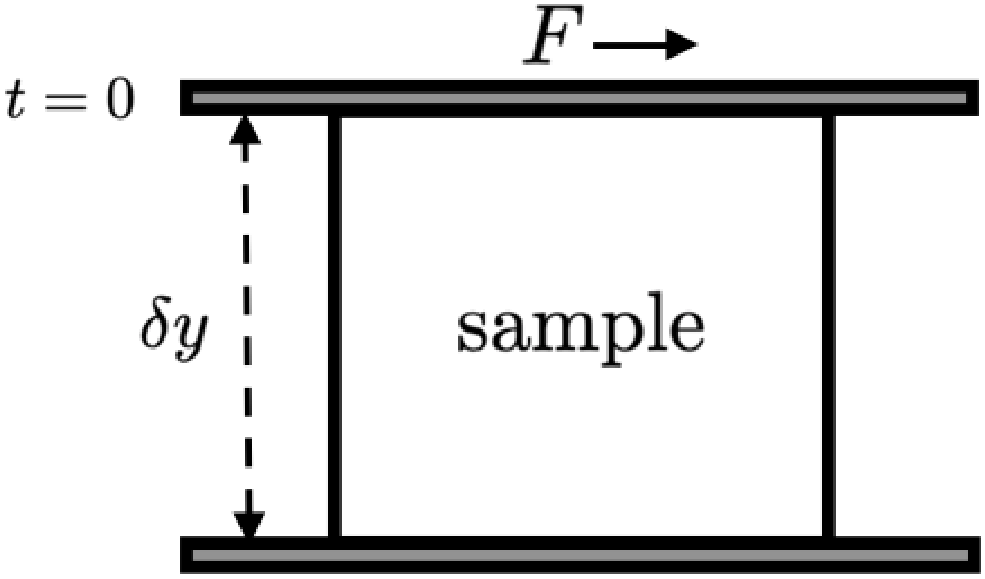
\includegraphics[width=6cm]{fig/shear-testing.png}
  \caption{A shear testing device (depicted in 2D).}
\end{figure}

\subsection{Shear in solids}

Consider the sample in our shear testing device is a solid, \figref{fig:shear-solids} shows the deformation after time $t'$. For any given shear $\tau$, the shear deformation is finite in solids. We can define a new quantity, shear strain $\lambda$, to measure this deformation:

\begin{equation}
  \lambda = \frac{ \Delta x }{ \delta y }
\end{equation}

\begin{figure} \label{fig:shear-solids}
  \centering
  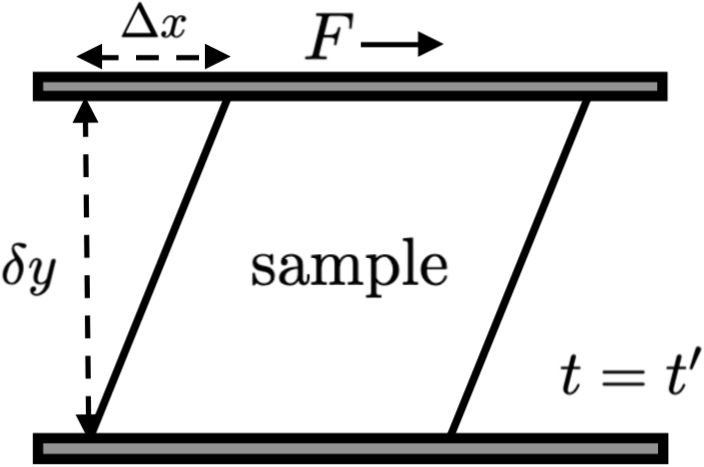
\includegraphics[width=6cm]{fig/shear-solid.png}
  \caption{Shear deformation at time $t'$ for a solid.}
\end{figure}

We can derive the relationship between shear stress and strain experimentally. In fact, it turns out they are related linearly. We call the constant of proportionality the Shear Modulus, $G$, and it is dependent on the material.

\begin{equation}\label{eq:shear-in-solids}
  \tau = G \lambda
\end{equation}

\subsection{Shear in fluids}

$~~~ t = t_1 ~~~ t = t_2 $
